\subsection{Compiler vs. Interpreters}
\begin{frame}{\textbf{Compiler vs. Interpreters}}
    \begin{figure}
        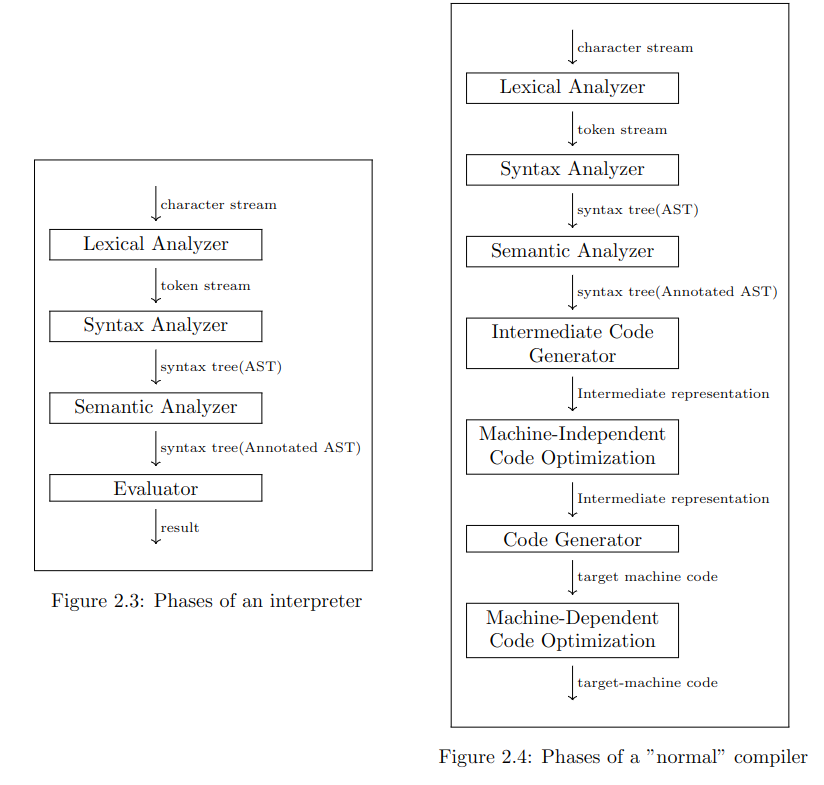
\includegraphics[scale=0.30]{Interpreter vs. Compiler.png}   
    \end{figure}
\end{frame}


\begin{frame}{\textbf{NB! IMPORTANT}}
    \begin{alertblock}{Compilers vs Interpreters!}
        We often end up using the term Compiler to talk about both Compilers and Interpreters, this is because they are very similar.\\
        This course deals exclusively with interpreters so unless stated otherwise assume that we are talking about interpreters.
    \end{alertblock}
    \begin{alertblock}{Expr vs AST}
        \begin{itemize}
            \item \textbf{Expr}: Expressions are terms that can be evaluated to a value, e.g. \texttt{1+2*3}
            \item \textbf{Stmt}: Statements are terms that are executed and result in a change of state. e.g. \texttt{var a = 1+2*3}
        \end{itemize}
    \end{alertblock}
\end{frame}

\subsection{Phases of an Interepreter}
\begin{frame}[fragile]{\textbf{Lexical Analysis}}
    \begin{block}{}
        \textbf{Lexical Analysis} breaks up strings into tokens. Also called a tokenizer.
    \end{block}
    \begin{example}
        \begin{figure}
            \centering
            \Large
            \begin{align*}
                (1+2)*13
            \end{align*}
        \end{figure}
        This gets tokenized into 
        \begin{lstlisting}[language=Haskell]
    ["(","1","+",2",")","*","13"]
        \end{lstlisting}
    \end{example}
\end{frame}
\subsection*{Phases of an Interepreter}
\begin{frame}{\textbf{Syntax Analyser}}
    \begin{example}
        \begin{figure}
            \centering
            \adjustbox{scale=0.7,center}{%
            \begin{tikzcd}
                \node[] (e0) {expr};
                \node[below left = of e0] (e1) {expr};
                \node[below left = of e1] (e11) {"("};
                \node[below = of e1] (e12) {expr};
                \node[below right = of e1] (e13) {")"};
                \node[below left = of e12] (e121) {number};
                \node[below = of e121] (e1211) {"1"};
                \node[below = of e12] (e122) {"+"};
                \node[below right = of e12] (e123) {number};
                \node[below = of e123] (e1231) {"2"};
                \node[below = of e0] (e2) {"*"};
                \node[below right = of e0] (e3) {number};
                \node[below = of e3] (e31) {"13"};
        
                \draw (e0) edge (e1)
                    (e0) edge (e2)
                    (e0) edge (e3)
                    (e1) edge (e11)
                    (e1) edge (e12)
                    (e1) edge (e13)
                    (e12) edge (e121)
                    (e12) edge (e122)
                    (e12) edge (e123)
                    (e121) edge (e1211)
                    (e123) edge (e1231);
        
            \end{tikzcd}
            }
        \end{figure}
    \end{example}
\end{frame}

\begin{frame}{\textbf{AST}}
    \begin{example}
        \begin{figure}[!h]
            \centering
            \adjustbox{scale=1,center}{%
            \begin{tikzcd}
                \node[] (e0) {\texttt{Mult}};
                \node[below left = of e0] (e1) {\texttt{Add}};
                \node[below left = of e1] (e11) {\texttt{1}};
                \node[below right = of e1] (e12) {\texttt{2}};
                \node[below right = of e0] (e2) {\texttt{13}};
        
                \draw (e0) edge (e1)
                    (e0) edge (e2)
                    (e1) edge (e11)
                    (e1) edge (e12);
            \end{tikzcd}
            }
        \end{figure}
    \end{example}
\end{frame}

\subsection{Semantic Analysis}
\begin{frame}{\textbf{Semantic Analyisis}}
    Semantic analysis lets us find out if the program is wellformed at find bugs at compile time, instead of at runtime.
    It also annotates the AST with certain information that's necessary for execution.

    \begin{block}{Wellformedness}
        For a program to be wellformed, we need to check for the following:
        \begin{itemize}
            \item \textbf{Type correctness}: The types of expressions in the program are correct.
            \item \textbf{Scope correctness}: The variables used in the program are declared.
            \item \textbf{Flow correctness}: The program is not stuck in an infinite loop.
            \item and more\dots
        \end{itemize}
        The first point is checked by a \textbf{type checker}.
    \end{block}
\end{frame}

\subsection{Type Checking}
\begin{frame}[fragile]{\textbf{Type Checking}}
    
    \begin{example}
        AST
        \lstinputlisting[language=Haskell, firstline=2, lastline=11]{examples/typecheck/typecheck.hs}
    \end{example}
\end{frame}
\subsection*{Type Checking}
\begin{frame}[fragile]{\textbf{Type Checking}}
    \begin{example}
        Types
        \lstinputlisting[language=Haskell, firstline=12, lastline=12]{examples/typecheck/typecheck.hs}
    \end{example}
\end{frame}

\begin{frame}[fragile]{\textbf{Type Checking}}
    \begin{example}
        \lstinputlisting[language=Haskell, firstline=14, lastline=21]{examples/typecheck/typecheck.hs}
    \end{example}
\end{frame}

\begin{frame}[fragile]{\textbf{Type Checking}}
    \begin{example}
        \lstinputlisting[language=Haskell, firstline=23, lastline=26]{examples/typecheck/typecheck.hs}
    \end{example}
\end{frame}

\begin{frame}[fragile]{\textbf{Type Checking}}
    \begin{example}
        \lstinputlisting[language=Haskell, firstline=28, lastline=31]{examples/typecheck/typecheck.hs}
    \end{example}
\end{frame}

\begin{frame}[fragile]{\textbf{Type Checking}}
    \begin{example}
        \lstinputlisting[language=Haskell, firstline=33, lastline=36]{examples/typecheck/typecheck.hs}
    \end{example}
\end{frame}

\begin{frame}[fragile]{\textbf{Type Checking}}
    \begin{example}
        \lstinputlisting[language=Haskell, firstline=38, lastline=41]{examples/typecheck/typecheck.hs}
    \end{example}
\end{frame}

\begin{frame}[fragile]{\textbf{Type Checking}}
    \begin{example}
        \lstinputlisting[language=Haskell, firstline=43, lastline=46]{examples/typecheck/typecheck.hs}
    \end{example}
\end{frame}

\begin{frame}[fragile]{\textbf{Type Checking}}
    \begin{example}
        \lstinputlisting[language=Haskell, firstline=48, lastline=48]{examples/typecheck/typecheck.hs}
    \end{example}
\end{frame}

\begin{frame}[fragile]{\textbf{Type Checking}}|
    \begin{example}
        \lstinputlisting[language=Haskell, firstline=50]{examples/typecheck/typecheck.hs}
    \end{example}
\end{frame}
\subsection*{Q\&A}
\begin{frame}{Questions?}
    \begin{figure}
        \centering
        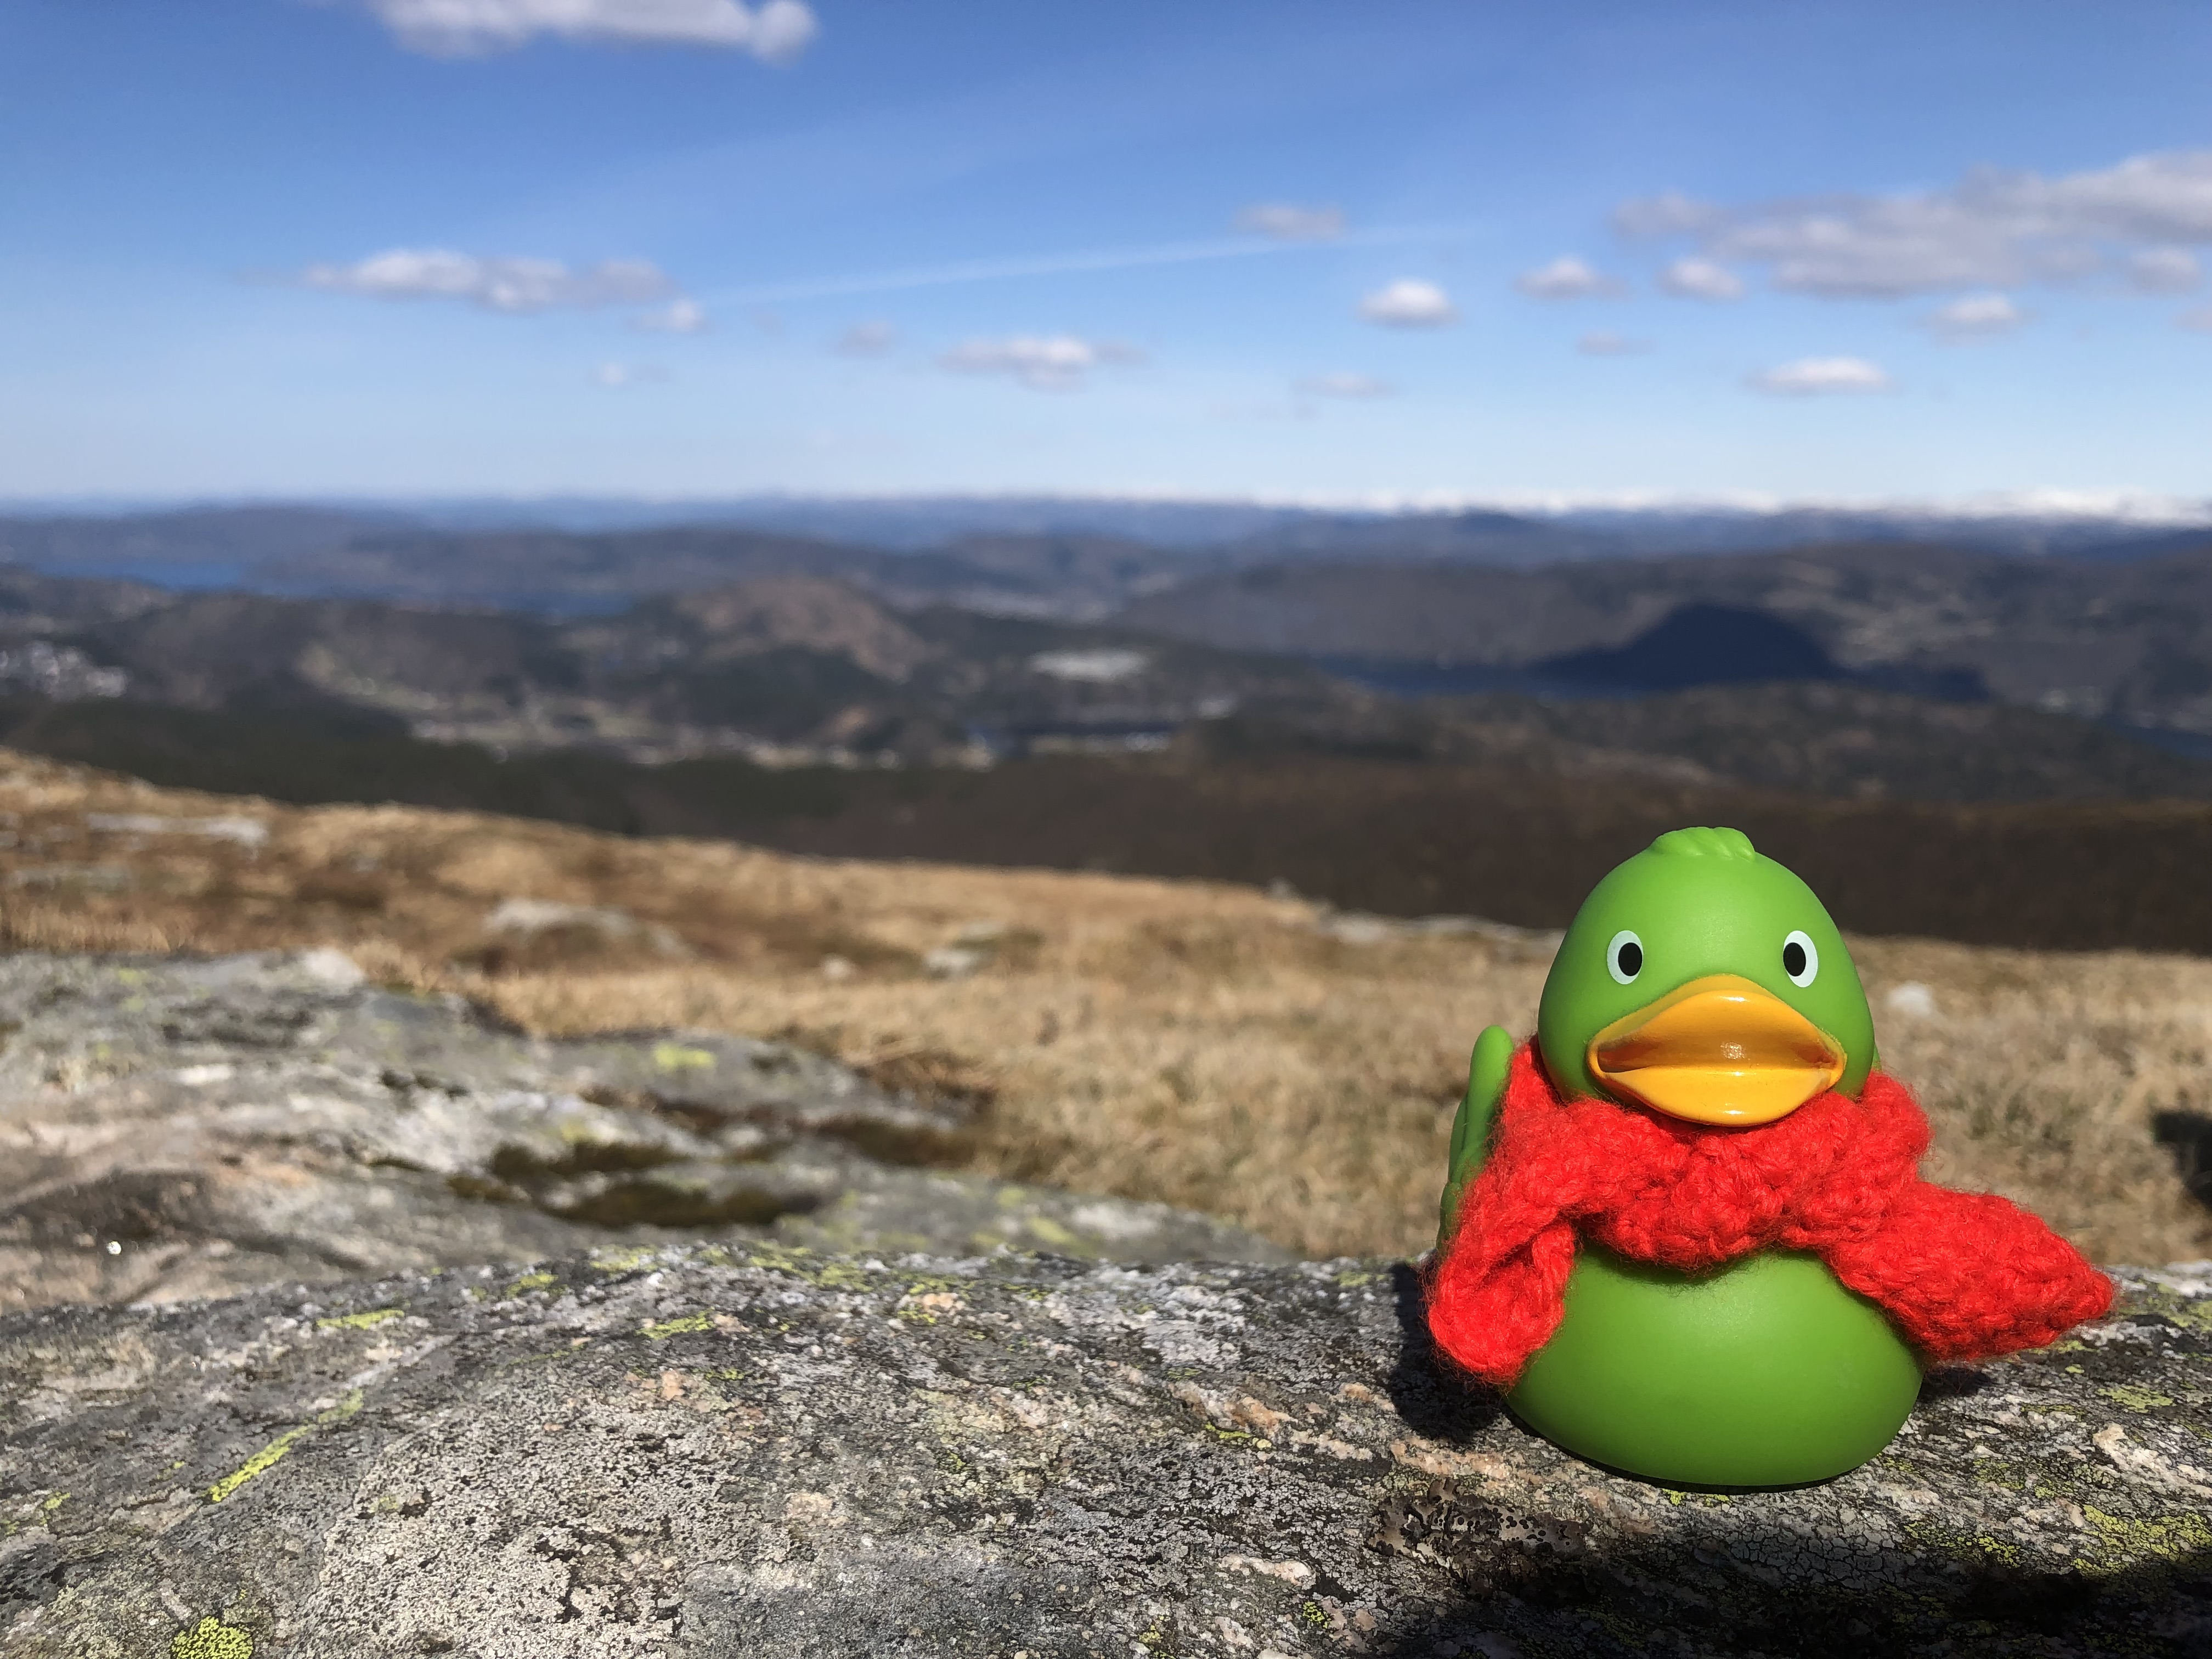
\includegraphics[height = 4.9cm]{guillaume3.jpg}
    \end{figure}
\end{frame}